In this section, we show that \LipCl are as powerful as any other classifier, like their unconstrained counterpart. In particular, when classes are separable they can achieve 100\% accuracy. % Even in the non separable case the optimal Bayes classifier can nonetheless be imitated. We also recall the main property of \mbox{1-Lipschitz} neural networks: their ability to produce robustness radius certificates against adversarial examples.  

\subsection{Boundary decision fitting}

    \begin{restatable}{proposition}{lippowerbinary}{\normalfont\textbf{Lipschitz Binary classification.}}\label{thm:lippowerbinary}
        For any binary classifier $c:\Xsub\rightarrow\Labels$ with closed pre-images ($c^{-1}(\{y\})$ is a closed set) there exists a 1-Lipschitz function $f:\Reals^n\rightarrow\Reals$ such that $\sign{(f(x))}=c(x)$ on $\Xsub$ and such that $\|\nabla_x f\|=1$ almost everywhere (w.r.t Lebesgue measure). 
    \end{restatable} %\todo{definition de la SDF en appendix avec citation ? \louis{Possible mais pas facile car l'exemple 3 en dépend.}}
    % (Proof, sketch) The function SDF($c$) introduced below in Definition~\ref{def:sdfsketch} verifies the aforementioned properties. Full proof in Appendix.  
    
    % \begin{definition}[Signed Distance Function]\label{def:sdfsketch}
    %     Let $\partial$ the frontier of maximum margin: the set of points equidistant to $c^{-1}(\{-1\})$ and $c^{-1}(\{+1\})$. We define the \textbf{Signed distance function (SDF)} as $\text{SDF}(c)(x)=c(x)d(x,\partial)$ on $\Xsub$, with $d$ the euclidean distance between a point and a set: $d(x,\partial)=\inf_{y\in\partial}d(x,y)$.
    % \end{definition}
      
    The level-sets of a $\text{Lip}_1(\Xsub,\Reals^K)$ functions (and especially the decision boundary) can be arbitrarily complex: restraining classifiers to $\text{Lip}_1(\Xsub,\Reals)$ does not affect the classification power. % Similar results can be obtained for multiclass classification (see Appendix). The \textbf{Error} of a classifier $c$ is defined as $E(c)=\Expect_{(x,y)\sim\Prob_{XY}}[\indicator\{c(x)\neq y\}]$.  % The \textbf{Risk} of a classifier is defined as $\Risk(c)=E(c)-E(b)$ where $b$ denotes the optimal Bayes classifier.  
    \begin{definition}[\textbf{$\epsilon$-separated distributions}]
    Distributions $P$ and $Q$ are $\epsilon$-separated if the distance between $\supp P$ and $\supp Q$ exceeds $\epsilon>0$.
    \end{definition}
    \begin{restatable}{corollary}{zeroerror}{\normalfont\textbf{Separable classes implies zero error}.}\label{thm:zeroerror}
        If $P$ and $Q$ are $\epsilon$-separated, then there exists a network $f\in\LipCl$ such that \textbf{error} $E(\sign\circ f)\coloneqq\Expect_{(x,y)\sim\Prob_{XY}}[\indicator\{\sign(f(x))\neq y\}]=0$.  
    \end{restatable} % \footnote{Practitioners sometimes prefer to monitor accuracy $1-E$.}
    
      The class of \LipCl networks does not suffer from bias for classification tasks. Some empirical studies show that indeed most datasets classes are separable~\cite{yang2020closer} such as CIFAR10 or MNIST. Furthermore, even if the classes are not separable, functions of \LipCl can nonetheless approximate the optimal Bayes classifier. Lipschitz constraint is not a constraint on the shape of the boundary (Figure~\ref{fig:signeddistancefunction}), but on the slope of the landscape of $f$. 
     
    % \begin{figure}[h]
    % \begin{minipage}{0.45\linewidth}
    % \begin{example}[Complex Decision Boundary]\label{fig:signeddistancefunction}
    %     We chose the boundary $\partial$ as the fourth iteration of Von Koch Snowflake. We chose $P$ as the interior ring, while the center and the exterior corresponds to $Q$. We train a $128\veryshortarrow 128\veryshortarrow 128\veryshortarrow 128\veryshortarrow 128$ \LipCl network with MSE to fit the SDF (Definition~\ref{def:nlctwoclasses} in Appendix) ground truth (160 000 pixels), until MAE is inferior to 1. It proves empirically that this classification task, associated to a very sharp (almost fractal) decision boundary, can be solved by a \LipCl network.   
    % \end{example}  % remove ?
    % \end{minipage}
    % \begin{minipage}{0.55\linewidth}
    % \centering
    %     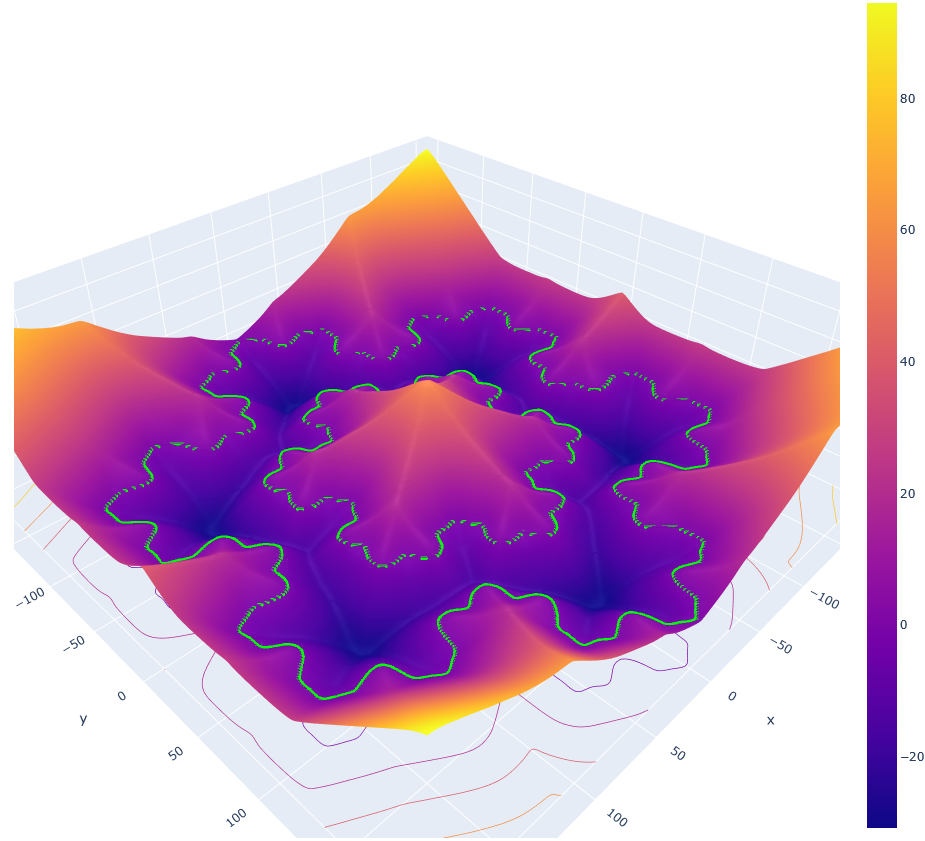
\includegraphics[width=0.7\linewidth]{images/toy/vonkoch_cropped.png}
    % \end{minipage}
    % \end{figure}
    
    \begin{figure}
     \centering
     \begin{subfigure}[b]{0.48\linewidth}
         \centering
         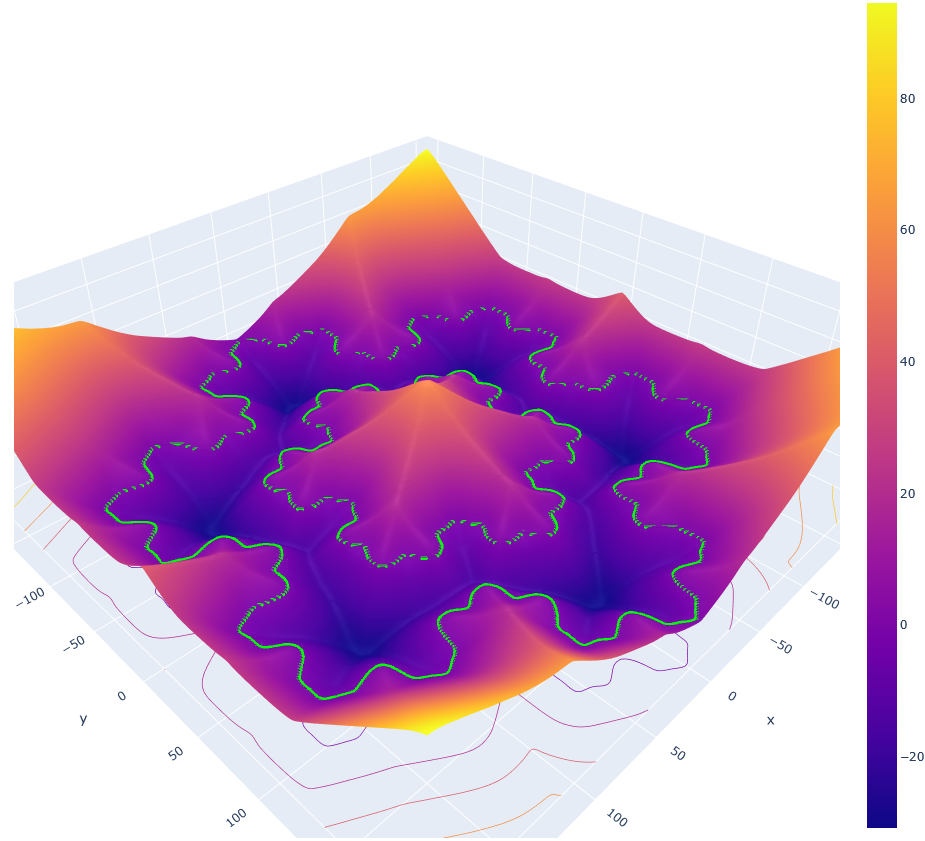
\includegraphics[width=0.9\linewidth]{images/toy/vonkoch_cropped.png}
         \caption{\textbf{Complex Decision Boundary $\partial$}. We chose $\partial$ as the fourth iteration of Von Koch Snowflake. We chose $P$ as the interior ring, while the center and the exterior correspond to $Q$. We train a \LipCl network with MSE to fit the SDF (Definition~\ref{def:nlctwoclasses} in Appendix) ground truth (160 000 pixels), until MAE is inferior to 1. It proves empirically that \LipCl networks can handle very sharp (almost fractal) decision boundary.}
         \label{fig:signeddistancefunction}
     \end{subfigure}
     \hfill
     \begin{subfigure}[b]{0.48\linewidth}
         \centering
         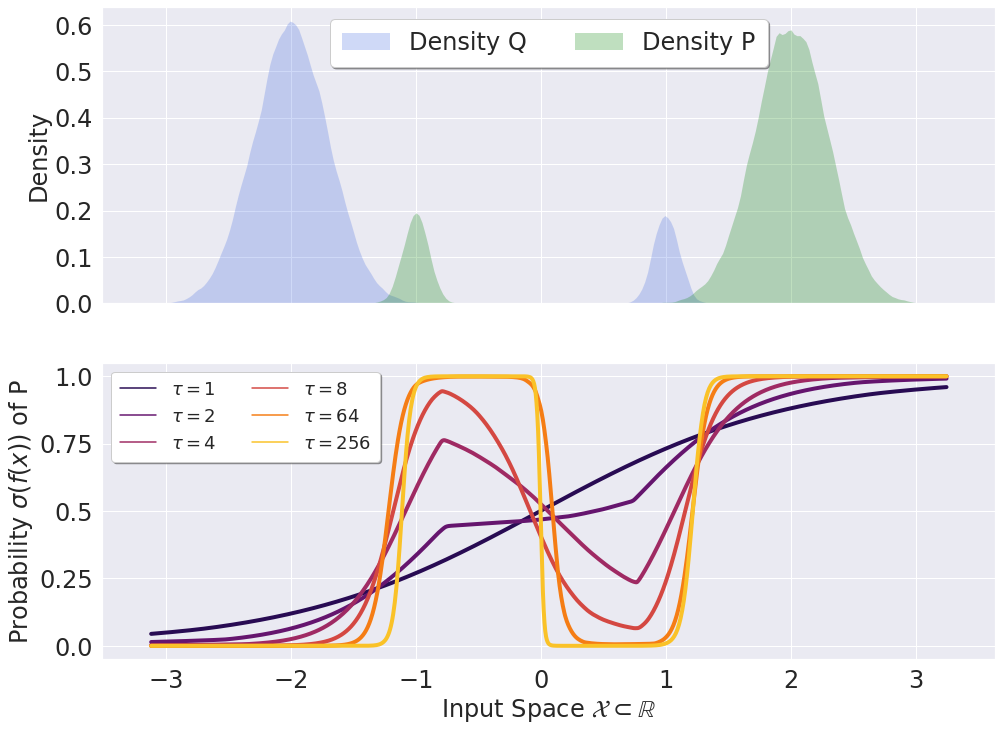
\includegraphics[width=1.\linewidth]{images/toy/toy_lip_overfit_splitted.png}
         \caption{\textbf{Importance of $\tau$ in BCE}. We train a \LipCl network with BCE and different values for $\tau$. We chose a toy example where $P$ and $Q$ are Gaussian mixtures with two modes of weights $0.9$ and $0.1$. We highlight the different shapes of the minimizer $\sigma\circ f$ as function of $\tau$. \textbf{High values of $\tau$ leads to better fitting, whereas for lower $\tau$ the small weights Gaussian of the mixture are treated as noise and ignored}.}
         \label{ex:nosameminimum}
     \end{subfigure}
     \caption{}
    \end{figure}
  

\subsection{Understanding why \LipCl are often perceived as not expressive}\label{sec:lipclminexists}

    \LipCl networks cannot reach zero loss with BCE: this may explain why they are perceived as not expressive enough. Yet the minimizer of BCE exists and is well defined.
    
    \begin{restatable}{proposition}{minimizerattained}{\normalfont\textbf{BCE minimization for \mbox{1-Lipschitz} functions}.}\label{thm:minimizerattained}
        Let $\Xsub\subset\Reals^n$ be a compact and $\tau>0$. Then the infimum in Equation~\ref{eq:optim1lip} is a minimum, denoted $f^{\tau}\in\text{Lip}_1(\Xsub,\Reals)$:
        \begin{equation}\label{eq:optim1lip}
            f^{\tau}\in\arg\inf_{f\in\text{Lip}_1(\Xsub,\Reals)}\Expect_{(x,y)\sim\Prob_{XY}}[\Loss^{bce}_{\tau}(f(x),y)].
        \end{equation}
         Moreover, the \LipCl networks will not suffer of vanishing gradient of the loss (see Appendix~\ref{app:gradientpreserving}).
    \end{restatable}
    
    Machine learning practitioners are mostly interested in maximizing accuracy.%the maximization of the accuracy.
    However, the minimizer of BCE is not necessarily a minimizer of the error (see Figure~\ref{ex:nosameminimum}). Yet, BCE is notoriously a differentiable proxy of the error $E(\sign\circ f)$, and as $\tau\rightarrow\infty$ we get asymptotically closer to maximum empirical accuracy. Bigger value for $\tau$ might ultimately lead to overfitting, playing the same role as the Lipschitz constant $L$ (see Figure~\ref{ex:nosameminimum}).  
    
    % \begin{figure}[h]
    % \begin{minipage}{0.55\linewidth}
    % \begin{example}\label{ex:nosameminimum}%[Importance of $L$ in BCE]
    %     We train a Lipschitz network with BCE and different values for $\tau$. We chose a toy example where $P$ and $Q$ are a Gaussian mixture with two modes of weights $0.9$ and $0.1$. We highlight the different shapes of the minimizer $\sigma\circ f$ as function of $\tau$. \textbf{High values of $\tau$ leads to better fitting, whereas for small $\tau$ the small weights Gaussian of the mixture are treated as noise and ignored}.   
    % \end{example}  % remove ?
    % \end{minipage}
    % \begin{minipage}{0.45\linewidth}
    % \centering
    %     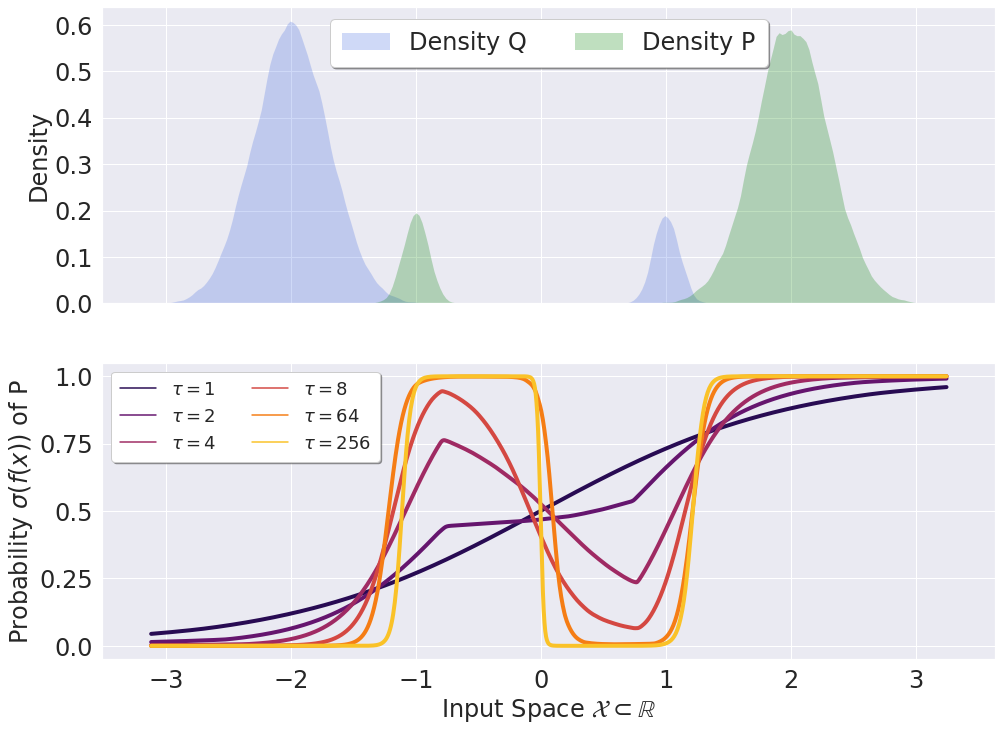
\includegraphics[width=0.9\linewidth]{images/toy/toy_lip_overfit_splitted.png}
    % \end{minipage}
    % \end{figure}
      
     \textbf{The implicit parameter $\tau=1$ of the loss is partially responsible of the poor accuracy of \LipCl networks in literature}, and not by any means the hypothesis space \LipCl itself. This can be observed in practice : when temperature $\tau$  (resp. margin $m$) of cross-entropy (resp. hinge loss) is correctly adjusted a small \LipCl CNN can reach a competitive \textbf{88.2\% validation accuracy on the CIFAR-10 dataset} (results synthetized and discussed in Figure~\ref{fig:pareto_hkr}) \textit{without} residual connections, batch normalization or dropout. Conversely, \LipInf networks are roughly equivalent to learning a \LipCl network with $\tau\rightarrow\infty$: without regularization or data augmentation, such a network can always reach 100\% train accuracy without generalization guarantees. %This phenomenon is illustrated in larger scale on CIFAR10, in Figure~\ref{fig:consistency}. \LipInf networks are equivalent to learning a \LipCl network with $\tau\rightarrow\infty$: without regularization or data augmentation, such a network can always reach 100\% train accuracy without generalization guarantees.  
    % \begin{figure}
    %     \centering
    %     % \begin{tabular}{lllllllllllllllllllllllll}
% \hline
% loss        &  CCE(0.001) &  CCE(0.01) &  CCE(0.05) &  CCE(0.1) &  CCE(30) &  CCE(2) &  CCE(0.5) &  CCE(1) &  CCE(3) &  CCE(5) &  CCE(10) &  hinge(100) &  hinge(50) &  hinge(36) &  hinge(20) &  hinge(10) &  hinge(0.005) &  hinge(2) &  hinge(0.5) &  hinge(1) &  hinge(0.01) &  hinge(0.3) &  hinge(0.05) &  hinge(0.1) \\
% \hline
% accuracy    &      0.4482 &     0.6666 &     0.7939 &    0.8311 &   0.8591 &   0.861 &    0.8619 &  0.8625 &  0.8688 &  0.8731 &   0.8768 &      0.6975 &     0.7489 &      0.768 &     0.8022 &     0.8335 &        0.8528 &    0.8632 &      0.8682 &    0.8715 &       0.8729 &      0.8759 &       0.8789 &      0.8827 \\
% prov\_acc\_36 &    0.389746 &   0.465234 &   0.254785 &  0.070508 &      0.0 &     0.0 &       0.0 &     0.0 &     0.0 &     0.0 &      0.0 &    0.436914 &   0.361719 &   0.290723 &   0.142969 &   0.009961 &           0.0 &       0.0 &         0.0 &       0.0 &          0.0 &         0.0 &          0.0 &         0.0 \\
% \hline
% \end{tabular}


\begin{tabular}{llrrrrrr}
\hline
          loss &  name &  accuracy &  certifiable\newline $\epsilon:36$ & certifiable\newline $\epsilon:72$ &  certifiable\newline $\epsilon:108$ &  prov\_avg\_rob &  MCR \\
\hline
    CCE(0.001) &   CCE &      0.45 &         0.39 &         0.34 &          0.29 &         90.52 &         -33.24 \\
     CCE(0.01) &   CCE &      0.67 &         0.47 &         0.29 &          0.15 &         47.40 &          30.78 \\
     CCE(0.05) &   CCE &      0.79 &         0.25 &         0.02 &          0.00 &         22.76 &          20.20 \\
      CCE(0.1) &   CCE &      0.83 &         0.07 &         0.00 &          0.00 &         14.87 &          13.65 \\
       CCE(30) &   CCE &      0.86 &         0.00 &         0.00 &          0.00 &          0.11 &           0.10 \\
        CCE(2) &   CCE &      0.86 &         0.00 &         0.00 &          0.00 &          1.26 &           1.20 \\
      CCE(0.5) &   CCE &      0.86 &         0.00 &         0.00 &          0.00 &          4.89 &           4.63 \\
        CCE(1) &   CCE &      0.86 &         0.00 &         0.00 &          0.00 &          2.82 &           2.67 \\
        CCE(3) &   CCE &      0.87 &         0.00 &         0.00 &          0.00 &          1.03 &           0.99 \\
        CCE(5) &   CCE &      0.87 &         0.00 &         0.00 &          0.00 &          0.63 &           0.60 \\
       CCE(10) &   CCE &      0.88 &         0.00 &         0.00 &          0.00 &          0.35 &           0.33 \\
 HKR(0.05,0.1) &   HKR &      0.36 &         0.33 &         0.30 &          0.27 &        113.89 &        -169.34 \\
   HKR(20,0.1) &   HKR &      0.36 &         0.33 &         0.29 &          0.27 &        113.19 &        -172.49 \\
   HKR(0.05,1) &   HKR &      0.39 &         0.35 &         0.31 &          0.28 &        113.10 &         -89.84 \\
     HKR(20,1) &   HKR &      0.40 &         0.36 &         0.32 &          0.28 &        115.45 &         -85.12 \\
   HKR(0.05,3) &   HKR &      0.50 &         0.41 &         0.34 &          0.29 &         92.68 &          17.66 \\
     HKR(20,3) &   HKR &      0.50 &         0.41 &         0.34 &          0.29 &         93.30 &          17.44 \\
   HKR(0.05,5) &   HKR &      0.56 &         0.44 &         0.34 &          0.26 &         76.22 &          37.84 \\
     HKR(20,5) &   HKR &      0.58 &         0.44 &         0.33 &          0.26 &         75.75 &          37.01 \\
  HKR(0.05,10) &   HKR &      0.64 &         0.41 &         0.28 &          0.18 &         51.40 &          36.96 \\
    HKR(20,10) &   HKR &      0.67 &         0.42 &         0.26 &          0.16 &         49.36 &          36.20 \\
  HKR(0.05,30) &   HKR &      0.74 &         0.24 &         0.06 &          0.01 &         20.55 &          18.01 \\
  HKR(0.05,50) &   HKR &      0.76 &         0.16 &         0.02 &          0.00 &         15.78 &          14.48 \\
    HKR(20,30) &   HKR &      0.78 &         0.30 &         0.07 &          0.01 &         25.92 &          22.67 \\
    HKR(20,50) &   HKR &      0.79 &         0.24 &         0.02 &          0.00 &         22.26 &          19.78 \\
   HKR(20,100) &   HKR &      0.80 &         0.21 &         0.01 &          0.00 &         20.49 &          18.30 \\
   HKR(20,300) &   HKR &      0.80 &         0.17 &         0.00 &          0.00 &         18.50 &          16.53 \\
 HKR(0.05,100) &   HKR &      0.82 &         0.01 &         0.00 &          0.00 &          5.19 &           4.96 \\
 HKR(0.05,300) &   HKR &      0.87 &         0.00 &         0.00 &          0.00 &          0.37 &           0.36 \\
HKR(0.05,1000) &   HKR &      0.88 &         0.00 &         0.00 &          0.00 &          0.23 &           0.23 \\
 HKR(0.05,500) &   HKR &      0.88 &         0.00 &         0.00 &          0.00 &          0.29 &           0.28 \\
    hinge(100) & hinge &      0.70 &         0.44 &         0.20 &          0.07 &         37.89 &          26.40 \\
     hinge(50) & hinge &      0.75 &         0.36 &         0.09 &          0.00 &         28.97 &          23.50 \\
     hinge(36) & hinge &      0.77 &         0.29 &         0.03 &          0.00 &         24.21 &          20.55 \\
     hinge(20) & hinge &      0.80 &         0.14 &         0.00 &          0.00 &         17.69 &          15.76 \\
     hinge(10) & hinge &      0.83 &         0.01 &         0.00 &          0.00 &         11.83 &          10.89 \\
  hinge(0.005) & hinge &      0.85 &         0.00 &         0.00 &          0.00 &          0.02 &           0.02 \\
      hinge(2) & hinge &      0.86 &         0.00 &         0.00 &          0.00 &          3.79 &           3.58 \\
    hinge(0.5) & hinge &      0.87 &         0.00 &         0.00 &          0.00 &          1.22 &           1.16 \\
      hinge(1) & hinge &      0.87 &         0.00 &         0.00 &          0.00 &          2.32 &           2.21 \\
   hinge(0.01) & hinge &      0.87 &         0.00 &         0.00 &          0.00 &          0.04 &           0.04 \\
    hinge(0.3) & hinge &      0.88 &         0.00 &         0.00 &          0.00 &          0.79 &           0.76 \\
   hinge(0.05) & hinge &      0.88 &         0.00 &         0.00 &          0.00 &          0.19 &           0.18 \\
    hinge(0.1) & hinge &      0.88 &         0.00 &         0.00 &          0.00 &          0.33 &           0.31 \\
\hline
\end{tabular}

    %     \caption{Caption}
    %     \label{fig:my_label}
    % \end{figure}
      
    %\footnote{}